\documentclass{beamer}
\usepackage[utf8]{inputenc}
\usepackage{tikz} % For semi-transparent background blocks
\usepackage{hyperref}
\usepackage{multimedia}
\usepackage{ulem}
\usepackage{wasysym}

\usepackage{pbox}

%%%%%%%%%%%%%%%%%%%%%%%%%%%%%%%%%%%%%%%%%%%%%%%%%%%%%%%%%%%%%%%%%%%
% Style modifications
%%%%%%%%%%%%%%%%%%%%%%%%%%%%%%%%%%%%%%%%%%%%%%%%%%%%%%%%%%%%%%%%%%%

\usetheme{Berlin}

%%% Fonts %%%

% Change font. Fontspec requires xelatex instead of pdflatex!
% Font catalog: http://www.tug.dk/FontCatalogue/
\usepackage{fontspec}

% Use "Fira Sans Light" as the normal font and the "Fira Sans" for
% bold fonts
\setsansfont[
  ItalicFont={Fira Sans Light Italic},
  BoldFont={Fira Sans},
  BoldItalicFont={Fira Sans Italic}]{Fira Sans Light}

\setbeamerfont{title}{size=\Large, series=\bfseries}
\setbeamerfont{frametitle}{size=\large, series=\bfseries}
\setbeamerfont{block body}{size=\Large}

%%% Slide template %%%

\setbeamertemplate{frames}[default]

% Empty headline / footline
\setbeamertemplate{headline}{}
\setbeamertemplate{footline}{}

% Remove navigation icons
\setbeamertemplate{navigation symbols}{}

%%% Colors %%%

\usecolortheme{crane}

\definecolor{lightgray}{RGB}{245,245,245}
\definecolor{darkgray}{RGB}{45,45,45}

\setbeamercolor{title}{fg=white,bg=darkgray}

\setbeamertemplate{blocks}[default]
\setbeamercolor{block title}{bg=}
\setbeamercolor{block body}{bg=lightgray}
\setbeamercolor{frametitle}{fg=white,bg=darkgray}
\setbeamercolor{itemize item}{fg=darkgray}
\setbeamertemplate{itemize items}[circle]
\setbeamercolor{section number projected}{bg=darkgray,fg=white}
\setbeamercolor{section in toc}{fg=darkgray}
\setbeamercolor{subsection in toc}{fg=darkgray}

\addtobeamertemplate{block begin}{\pgfsetfillopacity{0.8}}{\pgfsetfillopacity{1}}
\addtobeamertemplate{frametitle}{\pgfsetfillopacity{0.8}}{\pgfsetfillopacity{1}}
\addtobeamertemplate{title page}{\pgfsetfillopacity{0.8}}{\pgfsetfillopacity{1}}

%%% Misc %%%

% Command to place the test (e.g. citation) in the center of the footer
\newcommand{\setfootercentertext}[1]{
\setbeamertemplate{footline}{
  \hspace*{\fill}
  \raisebox{3mm}[0mm][0mm]{
    \tiny{#1}}\hspace*{\fill}}
}

%%%%%%%%%%%%%%%%%%%%%%%%%%%%%%%%%%%%%%%%%%%%%%%%%%%%%%%%%%%%%%%%%%%
% Content
%%%%%%%%%%%%%%%%%%%%%%%%%%%%%%%%%%%%%%%%%%%%%%%%%%%%%%%%%%%%%%%%%%%

%------------------------------------------------------------------------------
\title{What is good scientific practice\\for research software?}
%------------------------------------------------------------------------------

\subtitle{... and how can we make it part of our research culture?}

\author{\small Konrad U. Förstner\\
  \vspace{0.5cm}
  \href{http://twitter.com/konradfoerstner}{@konradfoerstner}}

\institute{University of Würzburg}

\date{\scriptsize May 10$^{th}$, 2017}

\logo{
  \href{https://creativecommons.org/licenses/by/4.0/}{
    
\includegraphics[width=0.88cm]{images/creative_commons_attribute.png}}}
\begin{document}
\begin{frame}{}
  \titlepage
\end{frame}
\logo{}

\setbeamertemplate{background}{}

% Symbiosis of technology and science
% Tools - Science
% examples: Telescope / Microscope
\begin{frame}
  \frametitle{}
  \begin{block}{}
    \begin{center}
      {\huge  Science $\rightleftarrows$ Technology}
      \end{center}
  \end{block}
\end{frame}

% Telescope
\setbeamertemplate{background}{
  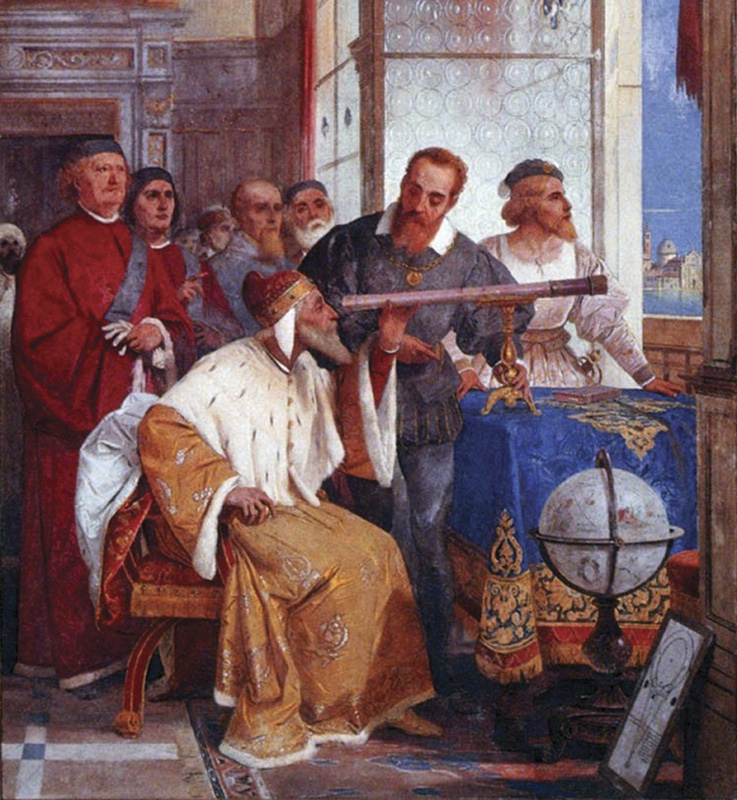
\includegraphics[width=\paperwidth]{images/Bertini_fresco_of_Galileo_Galilei_and_Doge_of_Venice.jpg}}
\setbeamertemplate{footline}{\raisebox{2mm}[2mm][2mm]{\Tiny{
      \href{https://commons.wikimedia.org/wiki/File:Bertini_fresco_of_Galileo_Galilei_and_Doge_of_Venice.jpg}{
        https://commons.wikimedia.org/wiki/File:Bertini\_fresco\_of\_Galileo\_Galilei\_and\_Doge\_of\_Venice.jpg} - PD}}}
\begin{frame}
\end{frame}

% Microscope
\setbeamertemplate{background}{
  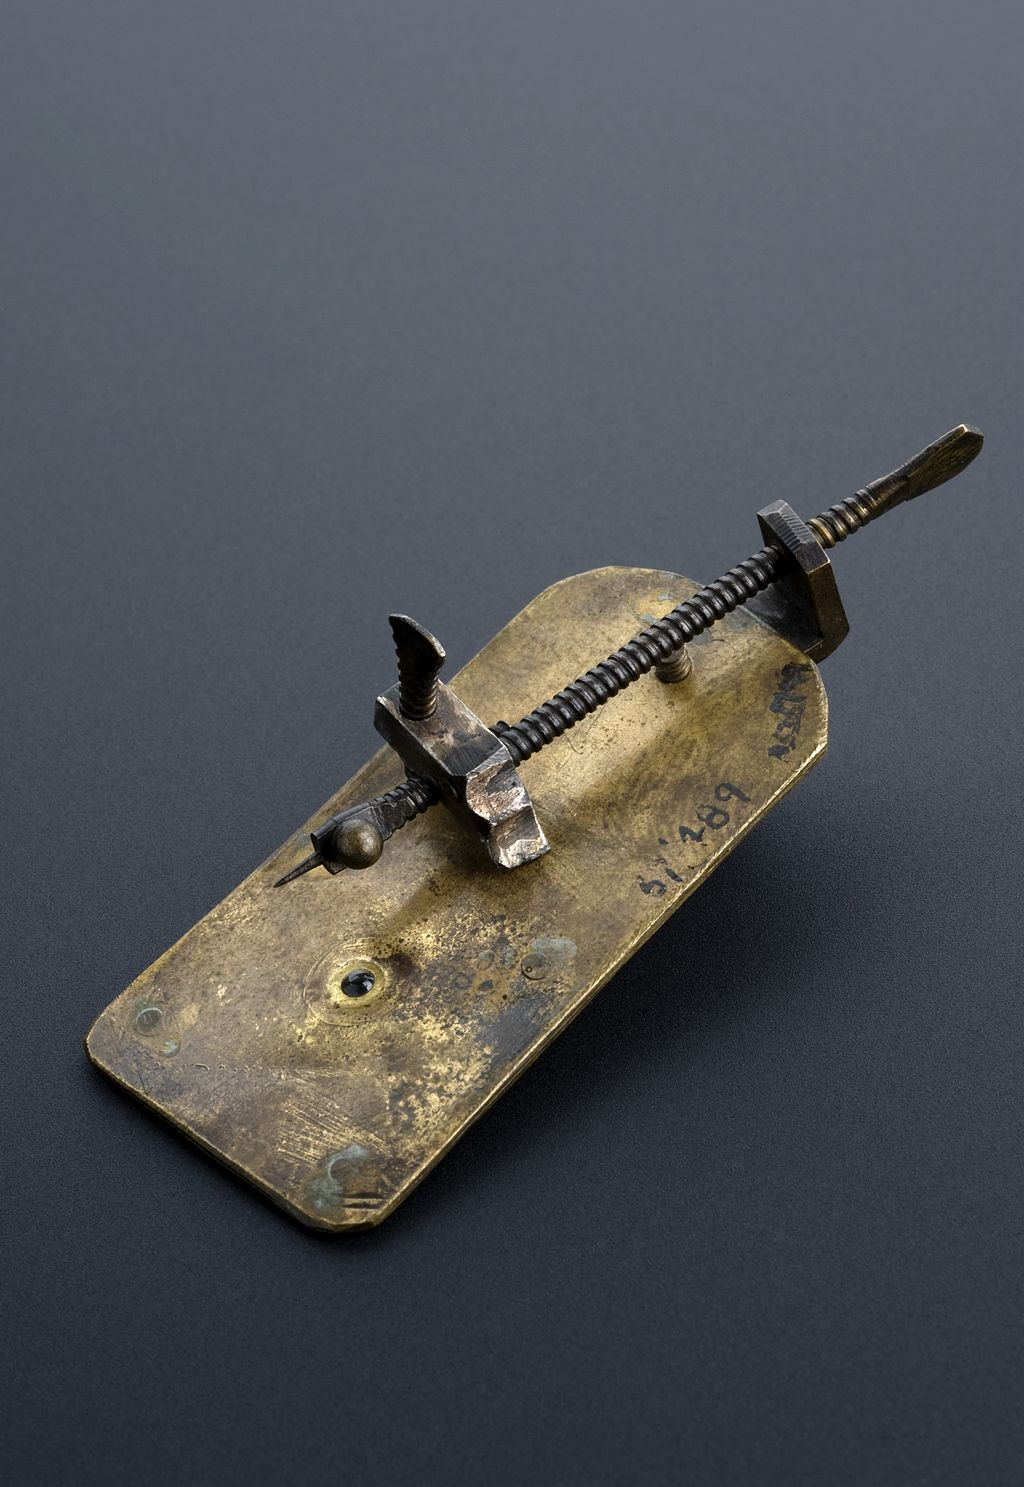
\includegraphics[width=\paperwidth,trim=0 0 0 110,clip]{images/1024px-Leeuwenhoek_simple_microscope_(copy),_Leyden,_1901-1930_Wellcome_L0057739.jpg}}
\setbeamertemplate{footline}{\raisebox{2mm}[2mm][2mm]{\Tiny{
      \href{https://commons.wikimedia.org/wiki/File:Leeuwenhoek_simple_microscope_(copy),_Leyden,_1901-1930_Wellcome_L0057739.jpg}{
        https://commons.wikimedia.org/wiki/File:Leeuwenhoek\_simple\_microscope\_(copy),\_Leyden,\_1901-1930\_Wellcome\_L0057739.jpg}
      - CC-By by Wiki Commons User \href{https://commons.wikimedia.org/wiki/User:Fæ}{Fæ}}}}
\begin{frame}
\end{frame}

% Sofware - ubiquitary 
\setbeamertemplate{background}{
  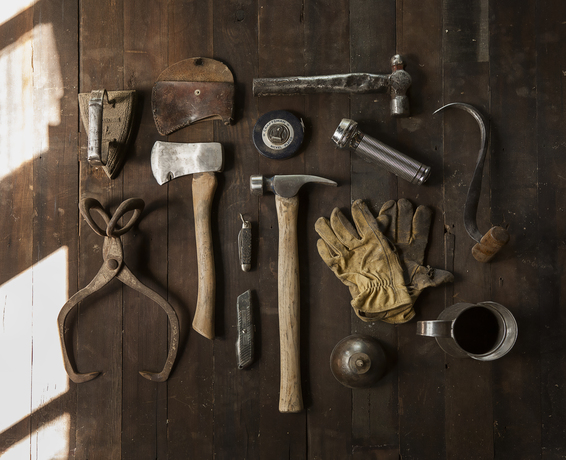
\includegraphics[width=\paperwidth]{images/Tools_by_Todd_Quackenbush.jpg}}
\setbeamertemplate{footline}{\raisebox{2mm}[2mm][2mm]{\Tiny{
      \href{https://unsplash.com/@toddquackenbush?photo=IClZBVw5W5A}{
        https://unsplash.com/@toddquackenbush?photo=IClZBVw5W5A} - PD}}}
\begin{frame}
  \pause  
  \begin{block}{}
    \begin{center}
      Software\\- an ubiquitous research tool
    \end{center}
  \end{block}  
\end{frame}

% Desktop application
\setbeamertemplate{background}{
  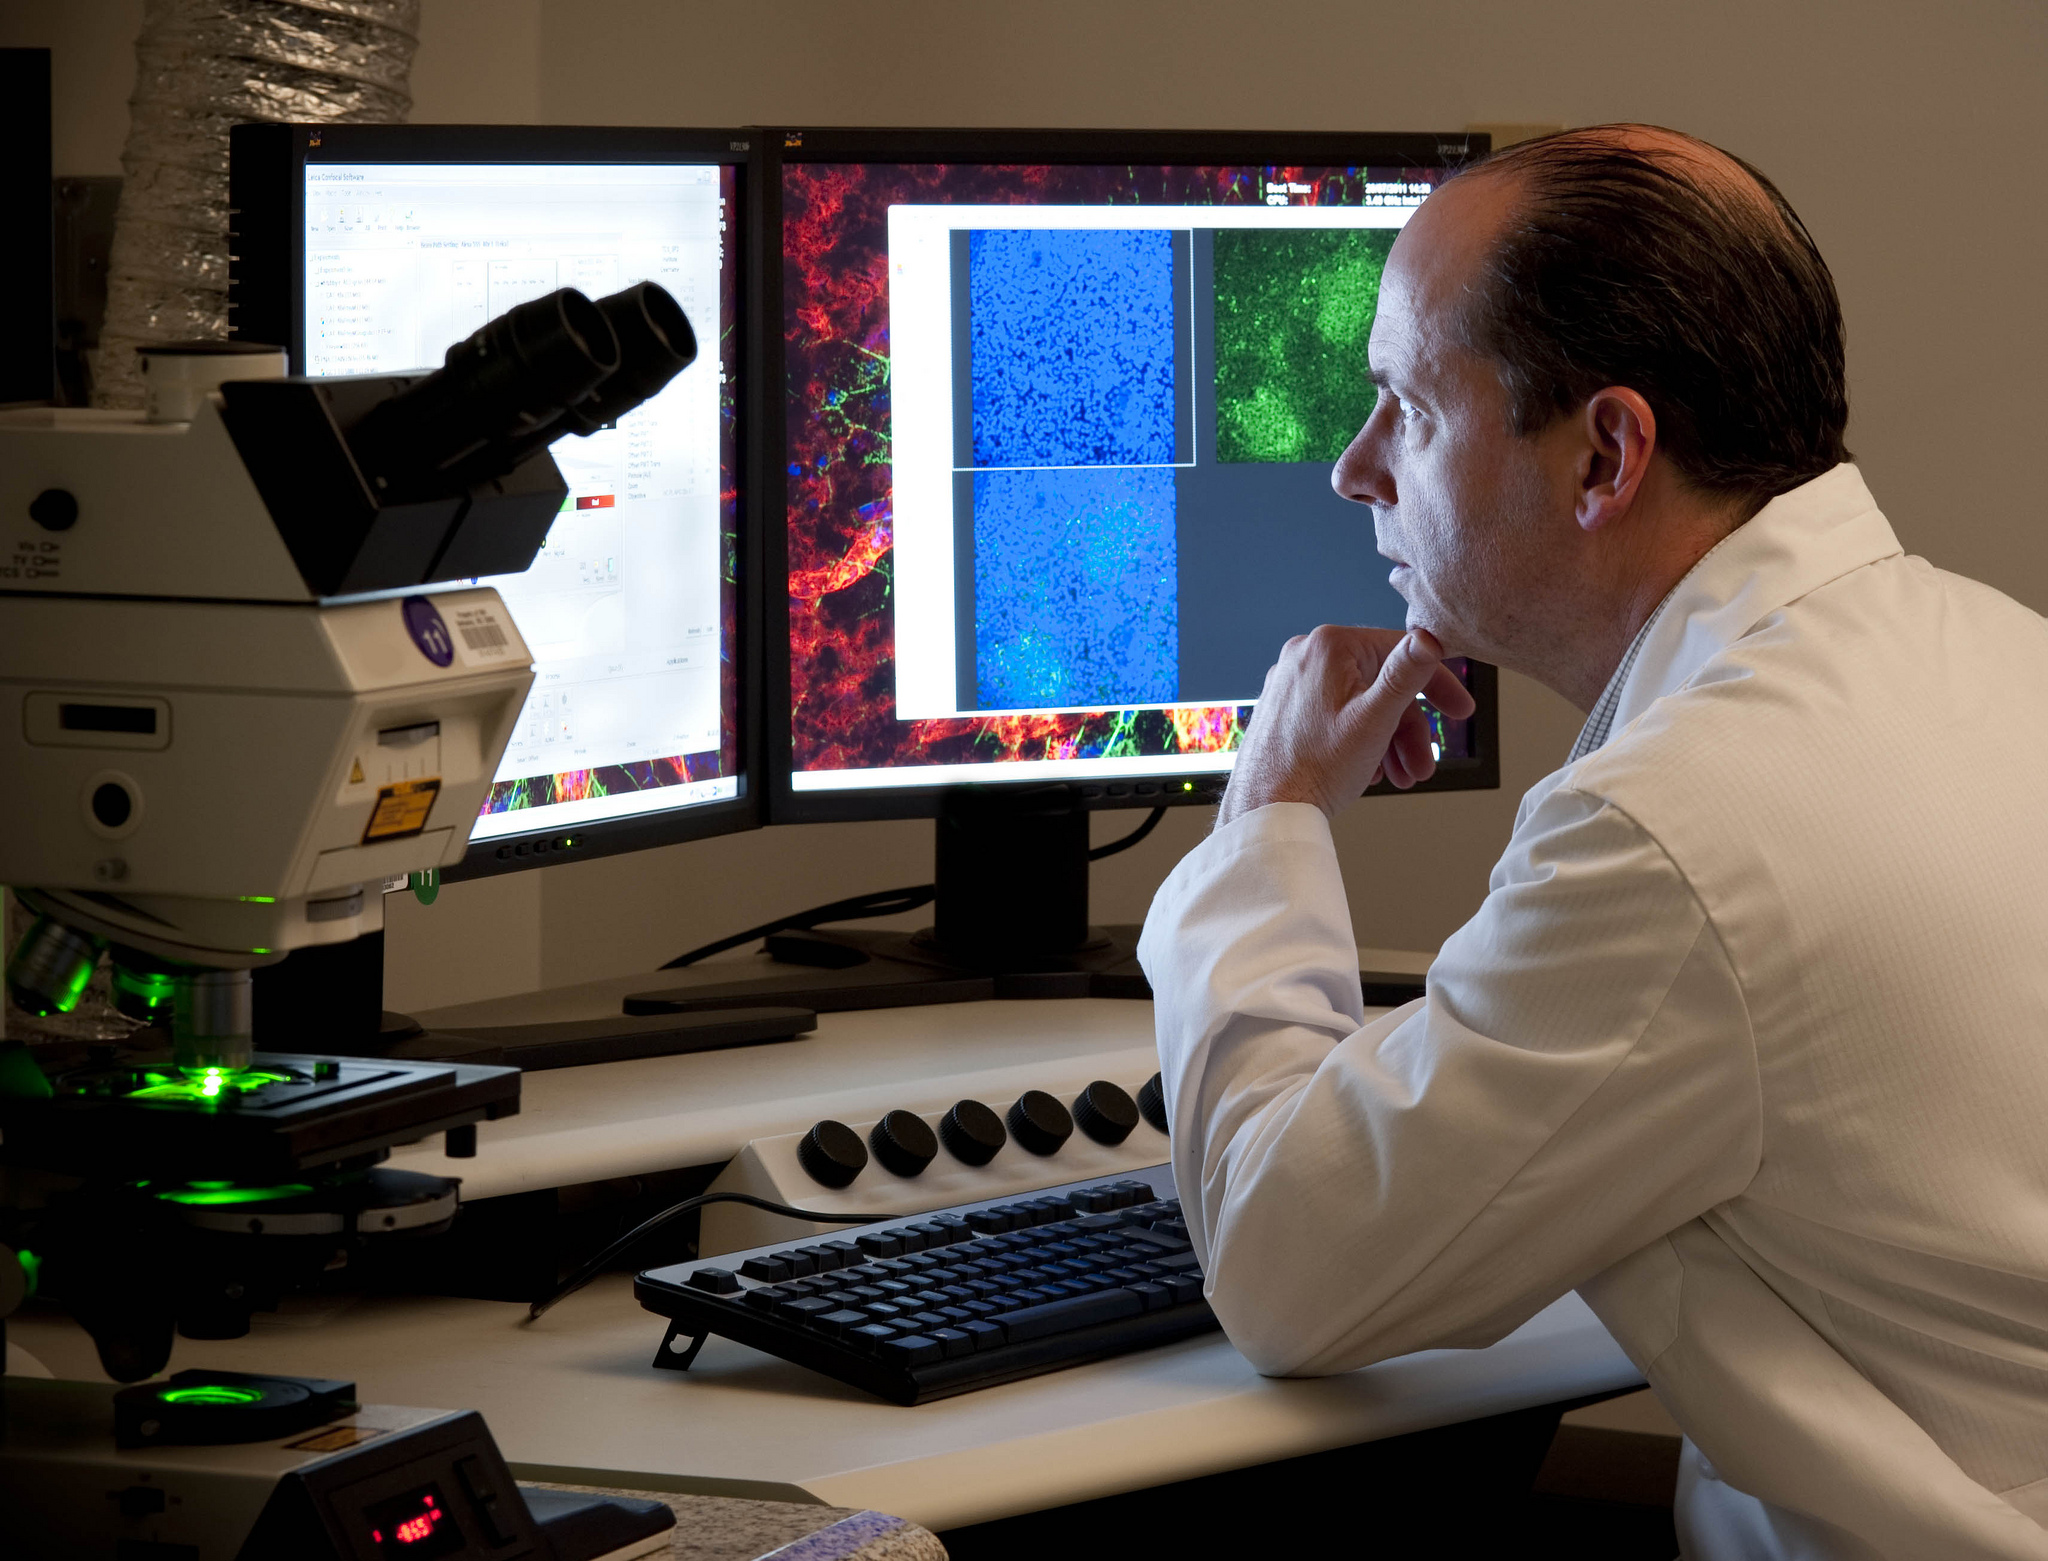
\includegraphics[width=\paperwidth]{images/Flickr_National_Eye_Institute_9955408263.jpg}}
\setbeamertemplate{footline}{\raisebox{2mm}[2mm][2mm]{\Tiny{https://www.flickr.com/photos/80030261@N06/9955408263}{
      https://www.flickr.com/photos/80030261@N06/9955408263}
    - CC-BY \href{https://www.flickr.com/photos/nationaleyeinstitute}{nationaleyeinstitute}}}
\begin{frame}
\end{frame}

% HPC calculation
\setbeamertemplate{background}{
  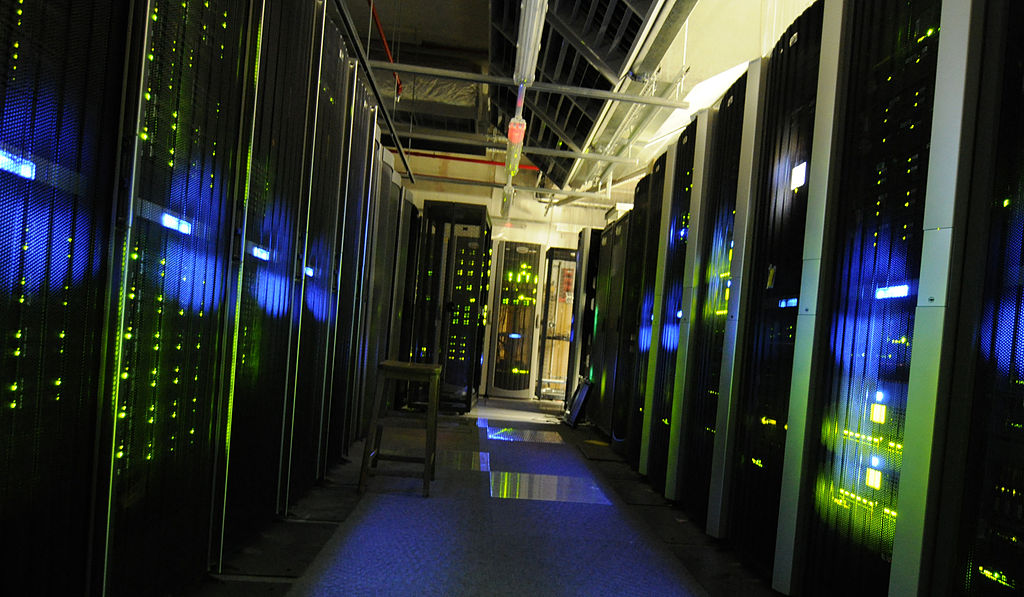
\includegraphics[height=\paperheight]{images/1024px-A_view_of_the_server_room_at_The_National_Archives.jpg}}
\setbeamertemplate{footline}{\raisebox{2mm}[2mm][2mm]{\Tiny{https://www.flickr.com/photos/80030261@N06/9955408263}{
      https://www.flickr.com/photos/80030261@N06/9955408263}
    - CC-By by Wiki Commons User \href{https://commons.wikimedia.org/w/index.php?title=User:EduVolunteer}{EduVolunteer}}}
\begin{frame}
\end{frame}

\setbeamertemplate{background}{}
\setbeamertemplate{footline}{}
\begin{frame}
  \frametitle{}
  \begin{block}{}
    \begin{center}
      It is unquestionable that there is a\\ strong and growing
      dependence of\\research on software.
      \end{center}
  \end{block}
\end{frame}


\setbeamertemplate{background}{}
\setbeamertemplate{footline}{}
\begin{frame}
  \frametitle{}
  \begin{block}{}
    \begin{center}
      Software is also a result of the\\ scientific
      work.\\\ \\ Quality, accessibility, citability, etc.\\
      have to be ensured.
      \end{center}
  \end{block}
\end{frame}

\setbeamertemplate{background}{}
\setbeamertemplate{footline}{}
\begin{frame}
  \frametitle{}
  \begin{block}{}
    \begin{center}
      The importance of software for research is widely ignored.
      \end{center}
  \end{block}
\end{frame}

\setbeamertemplate{background}{}
\setbeamertemplate{footline}{}
\begin{frame}
  \frametitle{}
  \begin{center}
    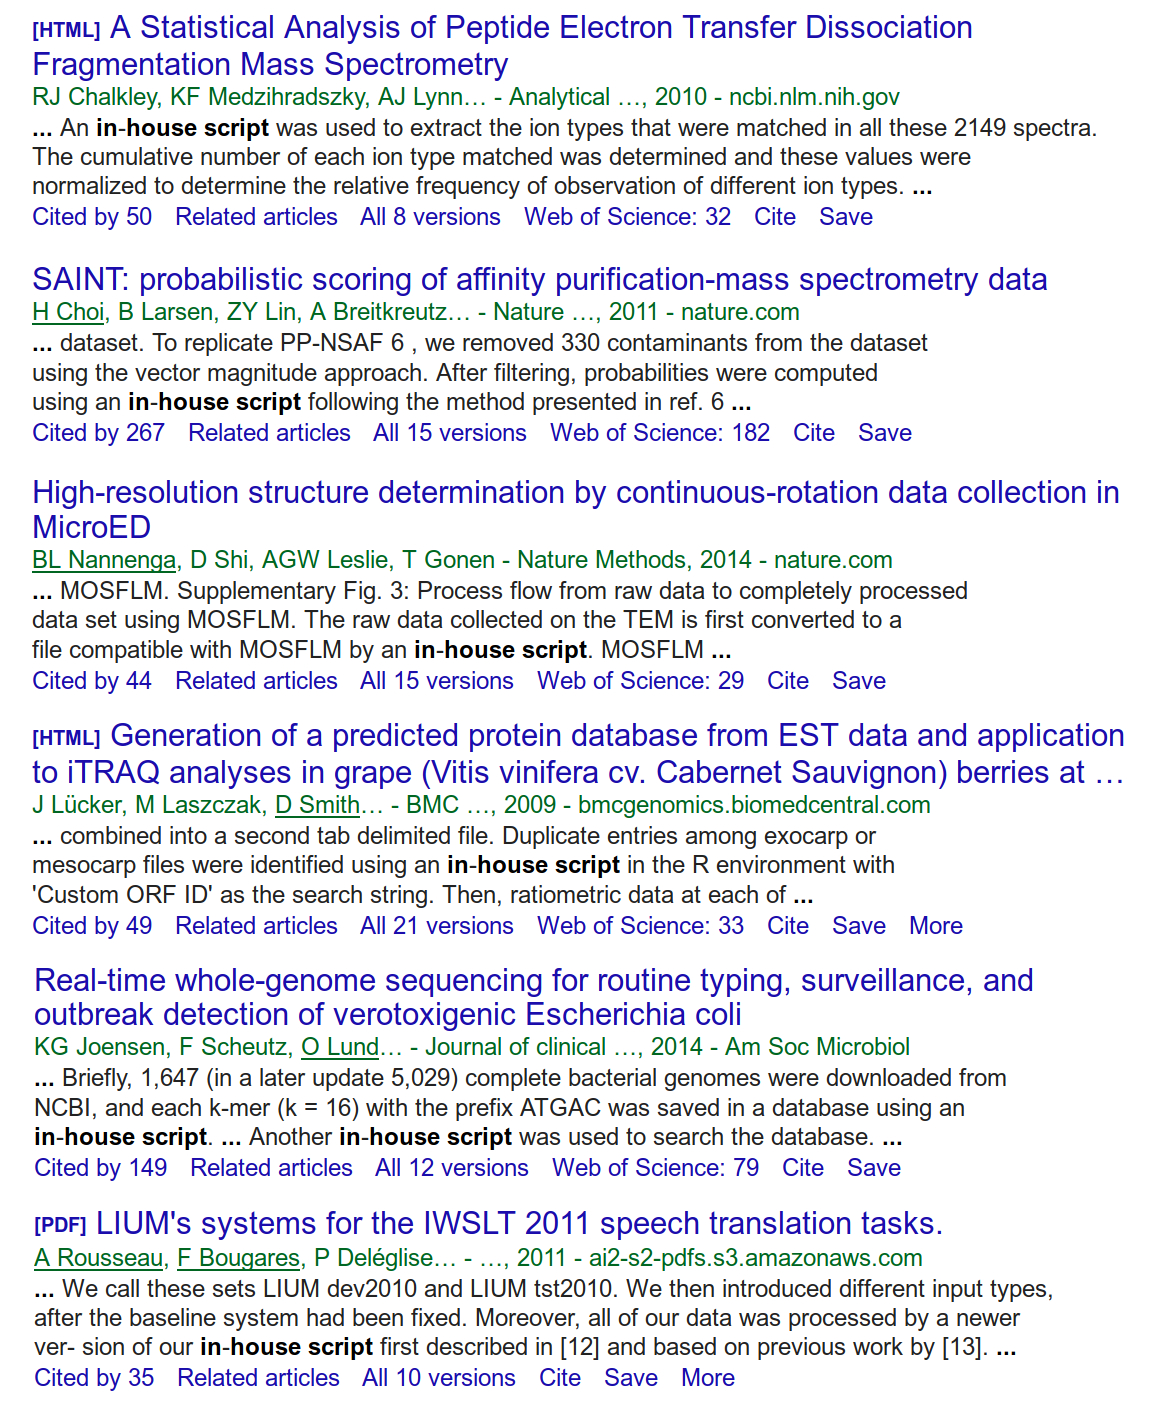
\includegraphics[height=9cm]{images/In-house_script.jpg}
  \end{center}
\end{frame}

\setbeamertemplate{background}{}
\setbeamertemplate{footline}{}
\begin{frame}
  \frametitle{}
  \begin{center}
    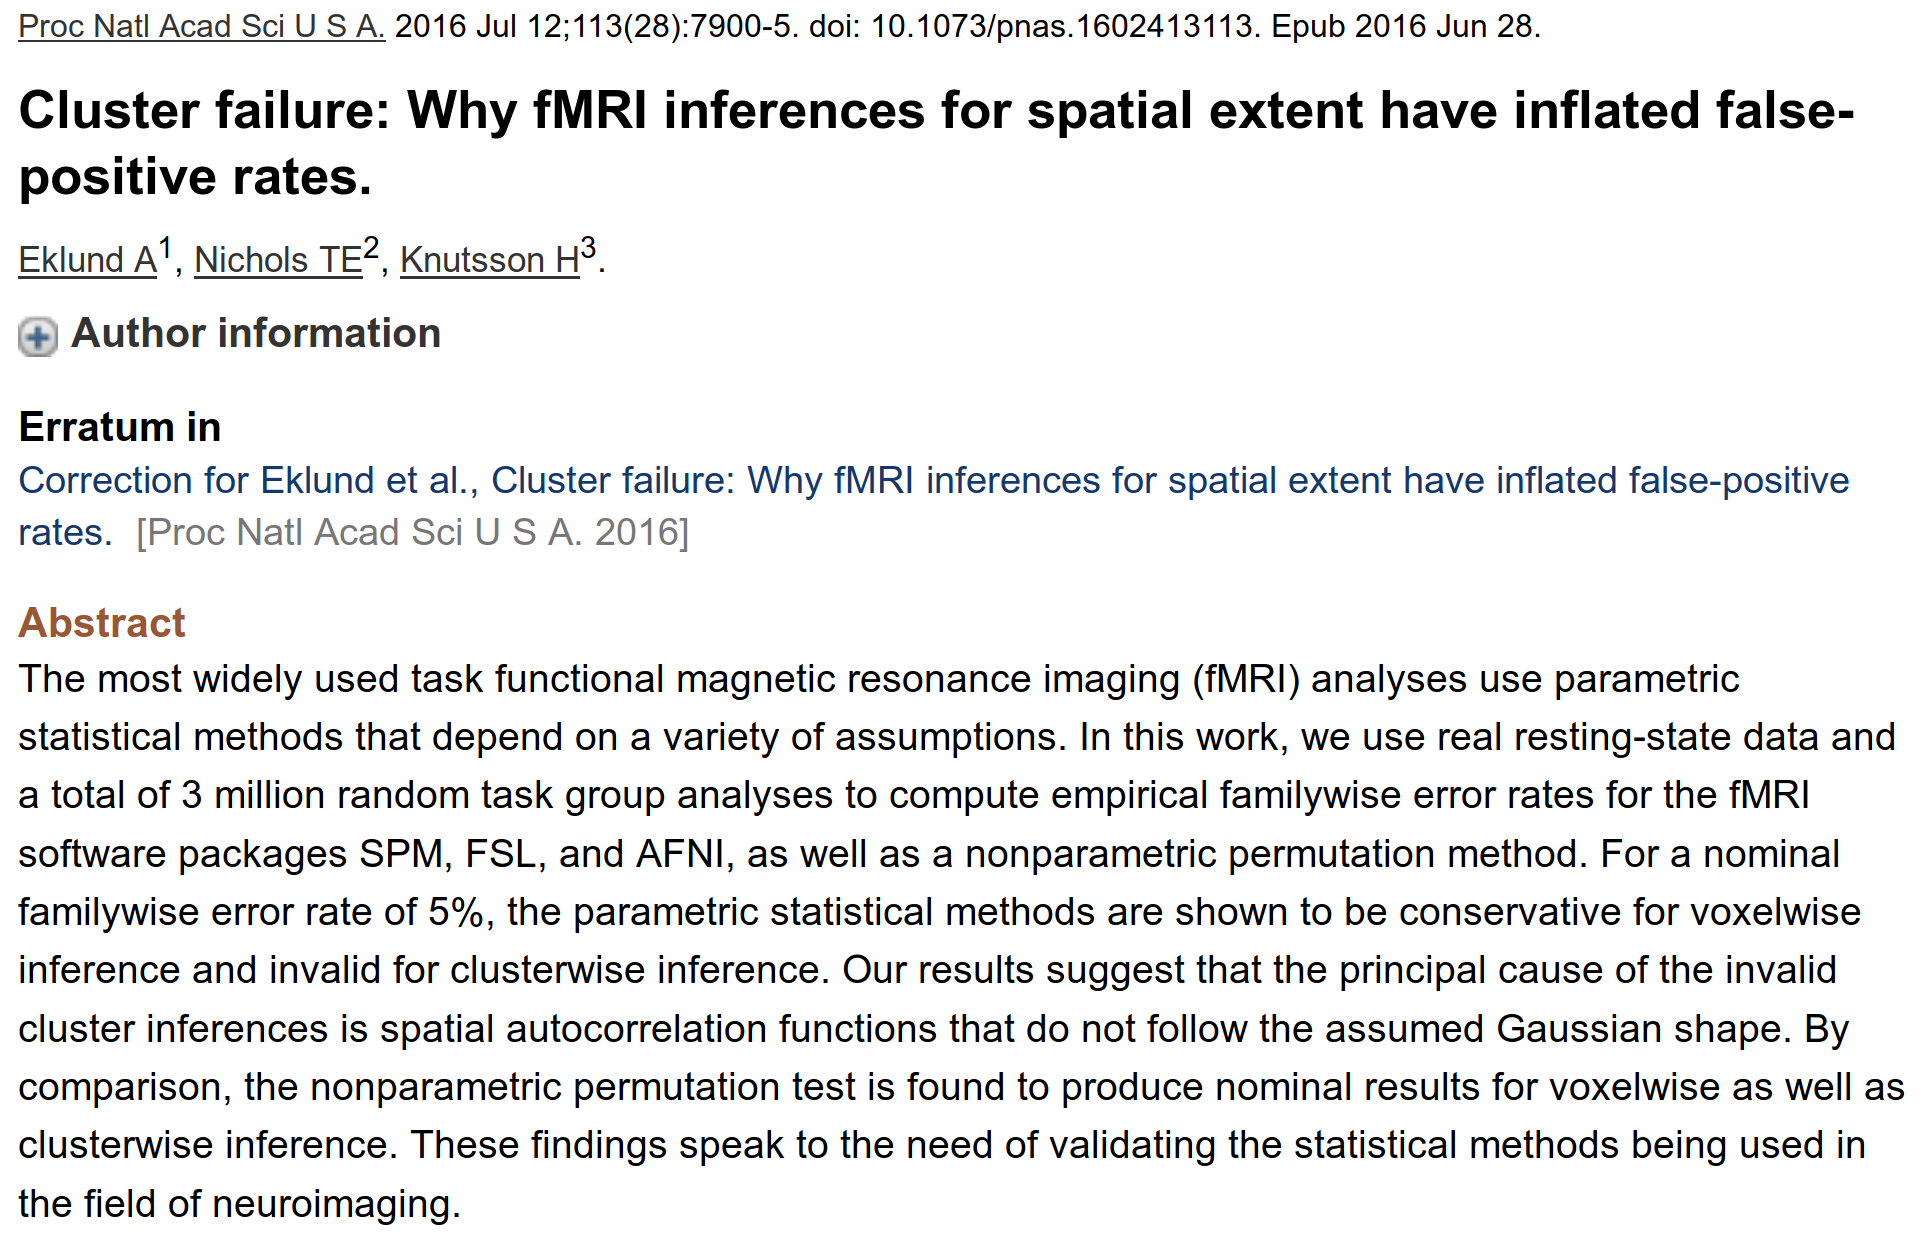
\includegraphics[height=7cm]{images/fMRI_software_failure.png}
  \end{center}
\end{frame}

\setbeamertemplate{background}{
  
\includegraphics[height=\paperheight]{images/Paris_Tuileries_Garden_Facepalm_statue.jpg}}
\setbeamertemplate{footline}{\raisebox{2mm}[2mm][2mm]{
    \Tiny \href{
      https://commons.wikimedia.org/wiki/File:Paris_Tuileries_Garden_Facepalm_statue.jpg}{
      https://commons.wikimedia.org/wiki/File:Paris\_Tuileries\_Garden\_Facepalm\_statue.jpg}
    - PD}}
\begin{frame}
  \frametitle{}
  \begin{block}{}
    \begin{center}
      Common problems with research software\\      
      \begin{itemize}
      \item Source code not published/available
      \item No quality control / automated tests
      \item Missing documentation
      \item Discontinued development (e.g. due to end of contract)
      \item Long-time availability not guaranteed        
      \item Missing citability
      \end{itemize}      
    \end{center}
  \end{block}
\end{frame}

\begin{frame}
  \frametitle{}
  \begin{block}{}
    \begin{center}
      Potential reasons\\
      \begin{itemize}
      \item Lack of awareness
      \item Lack of skills
      \item Lack of time
      \item Lack of incentives
      \item Lack of dedicated long-term funding
      \item No reviewing
      \item To hinder competitors
    \end{itemize}      
      \end{center}
  \end{block}
\end{frame}

% But this is changing, this confernce is a proof of this
% Several iniatives have been lauchend
\setbeamertemplate{background}{
  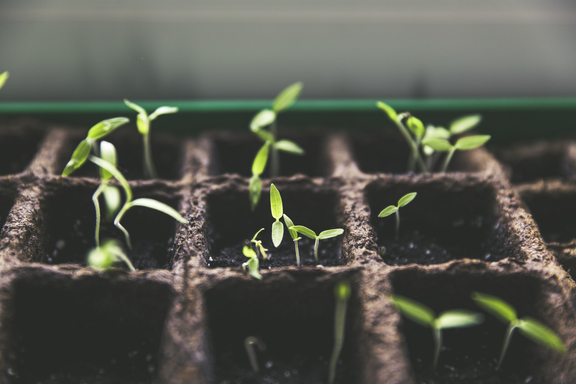
\includegraphics[height=\paperheight]{images/Sprout_by_Markus-Spiske.jpg}}
\setbeamertemplate{footline}{\raisebox{2mm}[2mm][2mm]{\Tiny{
      \href{https://unsplash.com/photos/vrbZVyX2k4I}{
        https://unsplash.com/photos/vrbZVyX2k4I} - PD}}}
\begin{frame}
  \begin{block}{}
    \begin{center}
      Several iniatives have been launched to address these issues.
    \end{center}
  \end{block}
\end{frame}


\begin{frame}
  \frametitle{}
  \begin{block}{}
    {\normalsize
      \begin{itemize}
      \item Software Carpentry (1998)\pause
      \item Software Sustainability Institute (2008)\pause
      \item WSSSPE (Working towards sustainable software for science:
        practice and experiences)\pause
      \item Free Software Foundation Europe published a position paper
        regarding research software\pause
      \item DANS (Data Archiving and Networked Services (DANS)\pause
      \item sciforge\pause
      \item DFG program "Research Software Sustainability"\\
        (7M €, 130 applications)\pause
      \item Helmholtz Association Task Group "Access to and re-use of
        research software" formed; organized a workshop about
        research software\pause
      \item de-RSE founded (\href{http://de-rse.org}{de-rse.org})\pause
      \item Several more ... lot of them here!
    \end{itemize}
    }
  \end{block}
\end{frame}

\setbeamertemplate{background}{}
\setbeamertemplate{footline}{
  \raisebox{2mm}[2mm][2mm]{\Tiny{\ The logos in this slide are excluded  from the CC-BY license statement}}}
\begin{frame}
  \frametitle{}
  \begin{center}
    Since 2008: Priority Initiative "Digital Information"\\  \ \\
    of the\\ \ \\
    Alliance of Science Organisations in Germany\\
    \ \\
    \includegraphics[height=2cm]{images/logo_allianz.png}\\
    \ \\
  \end{center}
\end{frame}

\setbeamertemplate{background}{}
\setbeamertemplate{footline}{}
\begin{frame}
  \frametitle{}
    \begin{block}{}
      \begin{center}
        Priority areas of the iniative\\
        \begin{itemize}
        \item Research Data
        \item Virtual Research Environments
        \item National Licensing
        \item National Hosting Strategy
        \item Legal Frameworks
        \item Open Access
        \end{itemize}
        \ \\ \ \\
        \pause Some fame due to the recent "DEAL" negotiations.
      \end{center}
    \end{block}
\end{frame}

\setbeamertemplate{background}{
  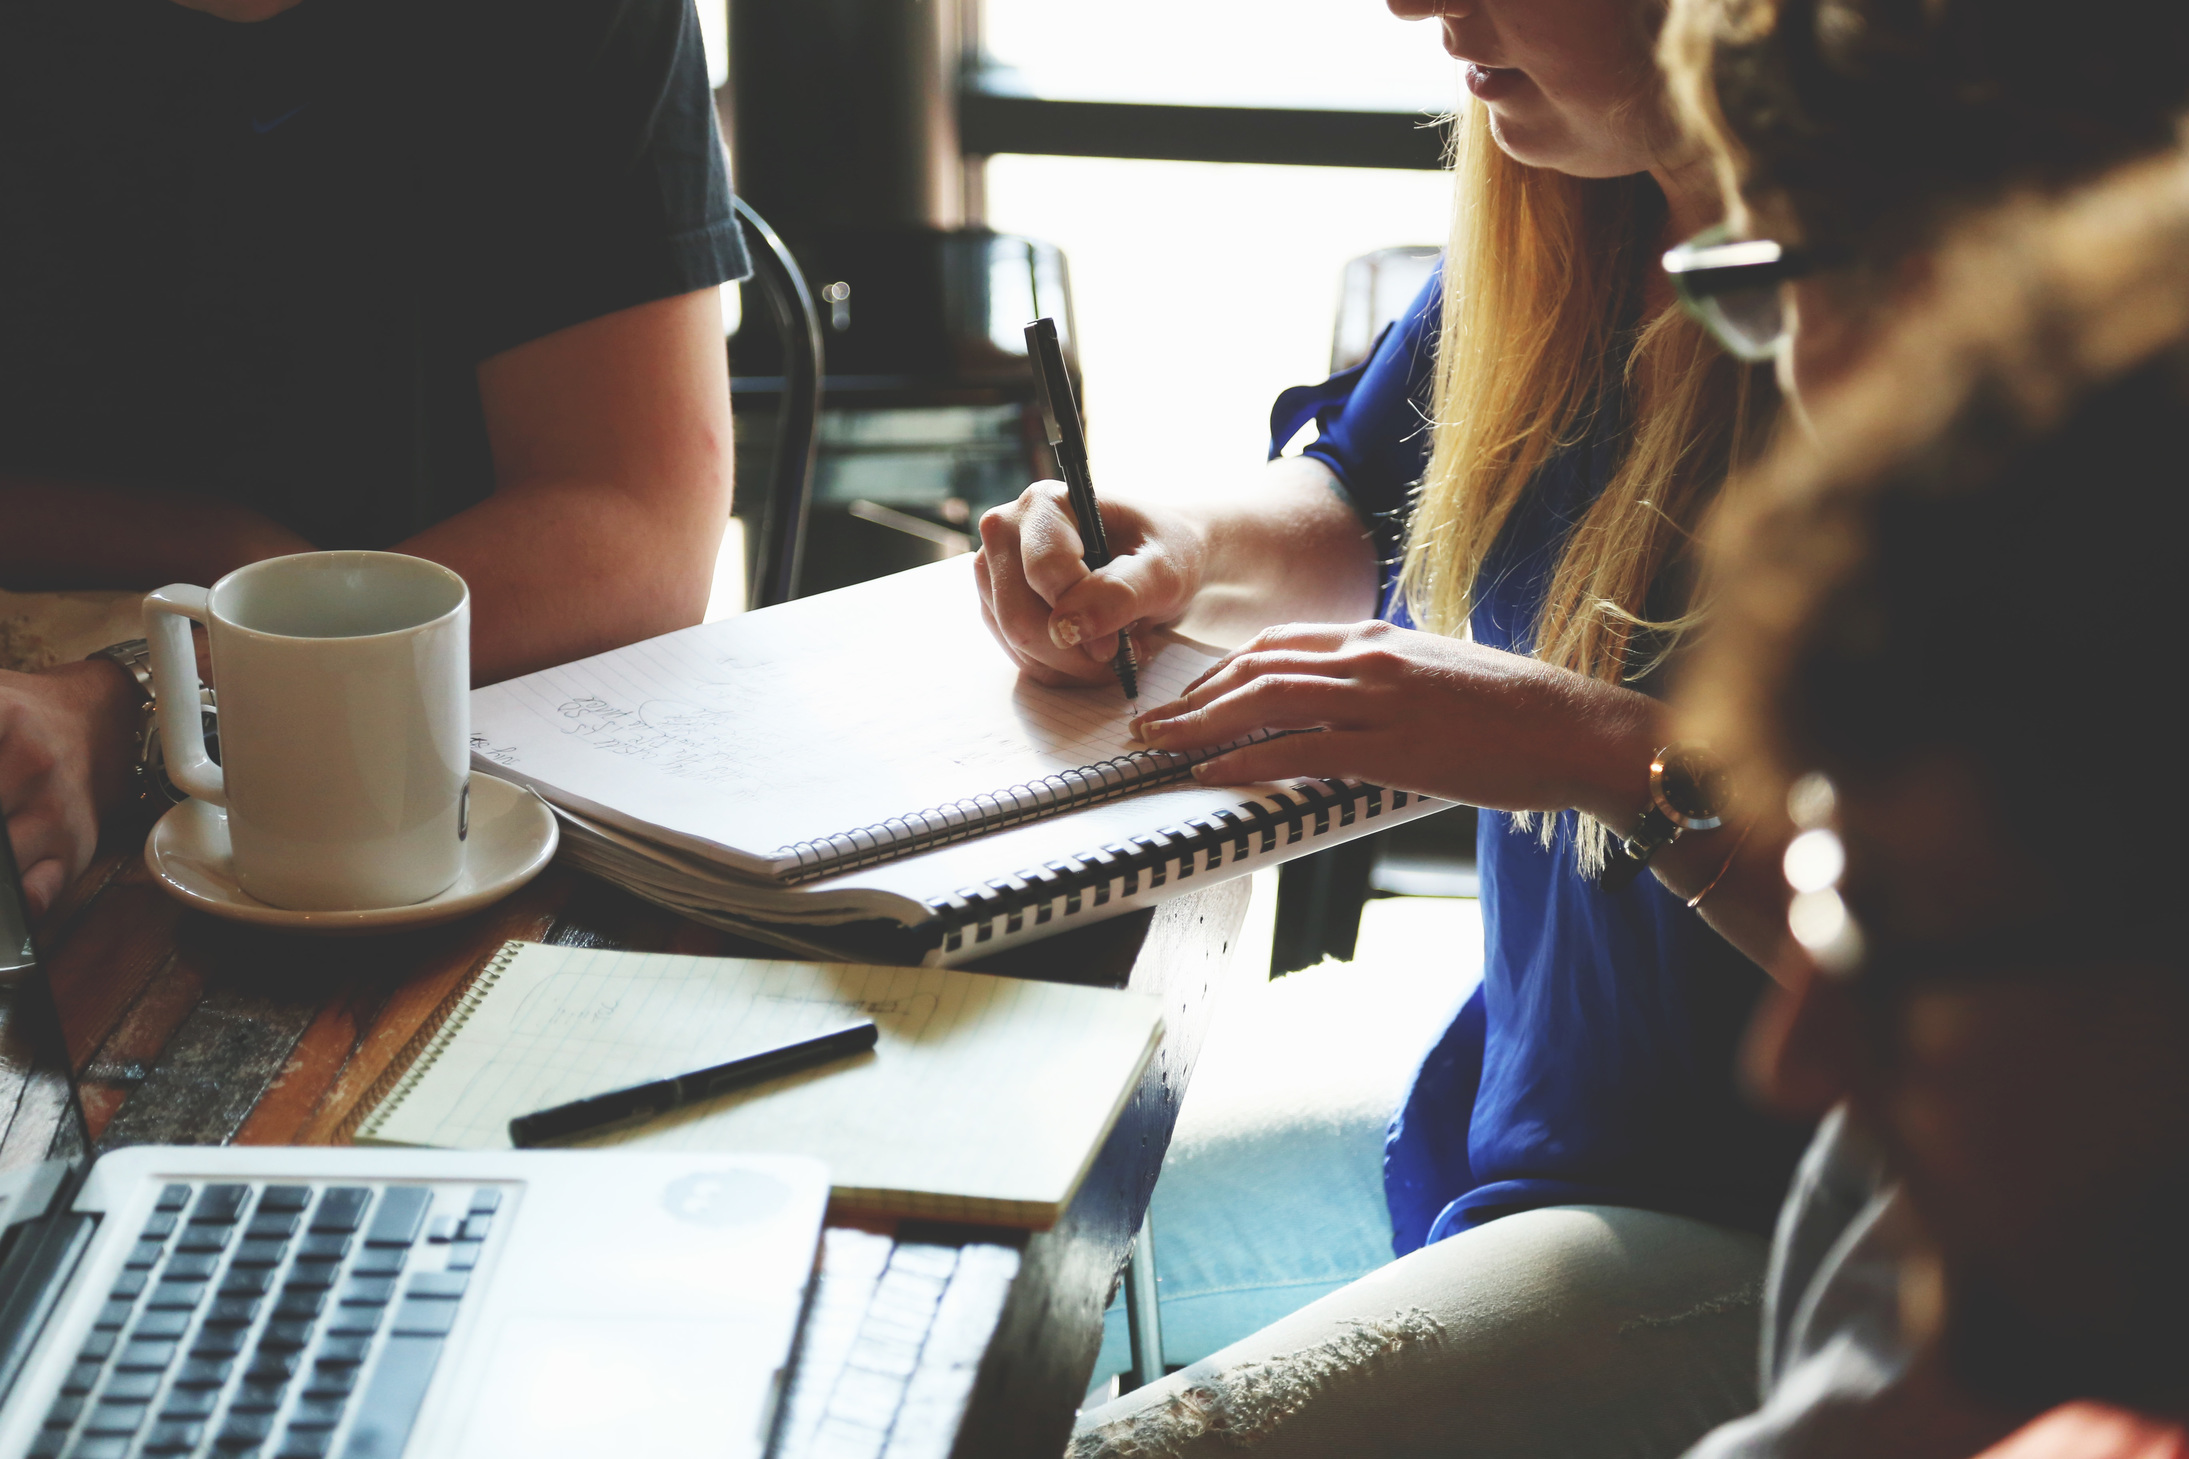
\includegraphics[height=\paperheight]{images/people-woman-coffee-meeting.jpg}}
\setbeamertemplate{footline}{\raisebox{2mm}[2mm][2mm]{\Tiny{
      \href{https://www.pexels.com/photo/people-coffee-meeting-team-7096/}{
        https://www.pexels.com/photo/people-coffee-meeting-team-7096/} - PD}}}
\begin{frame}
  \frametitle{}
    \begin{block}{}
      \begin{center}
        Since 2016\\ \ \\
        The cross-disciplinary \textit{ad-hoc} working group "Research Software"
      \end{center}
    \end{block}
\end{frame}

\begin{frame}
  \frametitle{}
    \begin{block}{}  
      \begin{center}
        {\large
      \begin{tabular}{lr}
        Mathias Bornschein & Ressortforschung des Bundes\\
        Dr. Matthias Katerbow & German Research Foundation \\
        Prof. Dr. Andreas Zeller & German Research Foundation\\
        Dr. Bernadette Fritzsch & Helmholtz Association \\
        Dr. Uwe Konrad & Helmholtz Association\\
        Dr. Georg Feulner & Leibniz Association\\
        Dr. Jürgen Fuhrmann & Leibniz Association\\
        Michael Franke & Max Planck Society \\
        Stephan Janosch & Max Planck Society \\
        Dr. Michael Erben-Russ & Fraunhofer Society \\
        Dennis Zielke & Fraunhofer Society \\        
        Prof. Dr. Björn Brembs & German Rectors' Conference\\
        Dr. Konrad Förstner & German Rectors' Conference\\
      \end{tabular}}
    \end{center}
    \end{block}
\end{frame}

\begin{frame}
  \frametitle{}
  \begin{block}{}
    \begin{center}
      The members have diverse backgrounds - scientist of different
      fields and\\scientific service / infrastructure providers.
    \end{center}
  \end{block}
\end{frame}

\begin{frame}
  \frametitle{}
  \begin{block}{}
    \begin{center}
      Our \textit{modus operandi}\\\ \\
      Compile recommendations and carry them back into our research
      organisations.
    \end{center}
  \end{block}
\end{frame}

\begin{frame}
  \frametitle{}
  \begin{block}{}
    \begin{center}
      Guiding principle\\\ \\
    The concept of Good Scientific Practice (GSP) must be also applied
    to research software.
    \end{center}
  \end{block}
\end{frame}

\begin{frame}
  \frametitle{}
  \begin{block}{}
    \begin{center}    
      But what can Good Scientific Practice mean\\ for research software?
      \end{center}       
  \end{block}
\end{frame}

\begin{frame}
  \frametitle{}
  \begin{block}{}
    \begin{center}
        \begin{itemize}
        \item Reproducibility
        \item Confirmability          
        \item Transparency
        \item Qualility
        \item Re-usability
        \end{itemize}
      \end{center}       
  \end{block}
\end{frame}

\begin{frame}
  \frametitle{}
  \begin{block}{}
    \begin{center}
      Our working model -- three types of software\\
      \begin{itemize}
      \item[1.] Small tools written for single purpose
      \item[2.] Software applications (as research output)
      \item[3.] Infrastructure and online services
      \end{itemize}
    \end{center}
  \end{block}
\end{frame}

\begin{frame}
  \frametitle{}
  \begin{block}{}
    \begin{center}
      All three levels are relevant and\\have to be addressed.
    \end{center}
  \end{block}
\end{frame}


\begin{frame}
  \frametitle{}
  \begin{block}{}
    \begin{center}
      Exact needs and possibilities might differ between scientific
      communities.\\\ \\
      Discourse must also happen\\inside of these  communities.
    \end{center}
  \end{block}
\end{frame}

\begin{frame}
  \frametitle{}
  \begin{block}{}
    \begin{center}
      E.g. what exactly means "reproducibility" (bit-identical
      compilation?) and how long would this needed to be guaranteed?
    \end{center}
  \end{block}
\end{frame}

\setbeamertemplate{background}{
  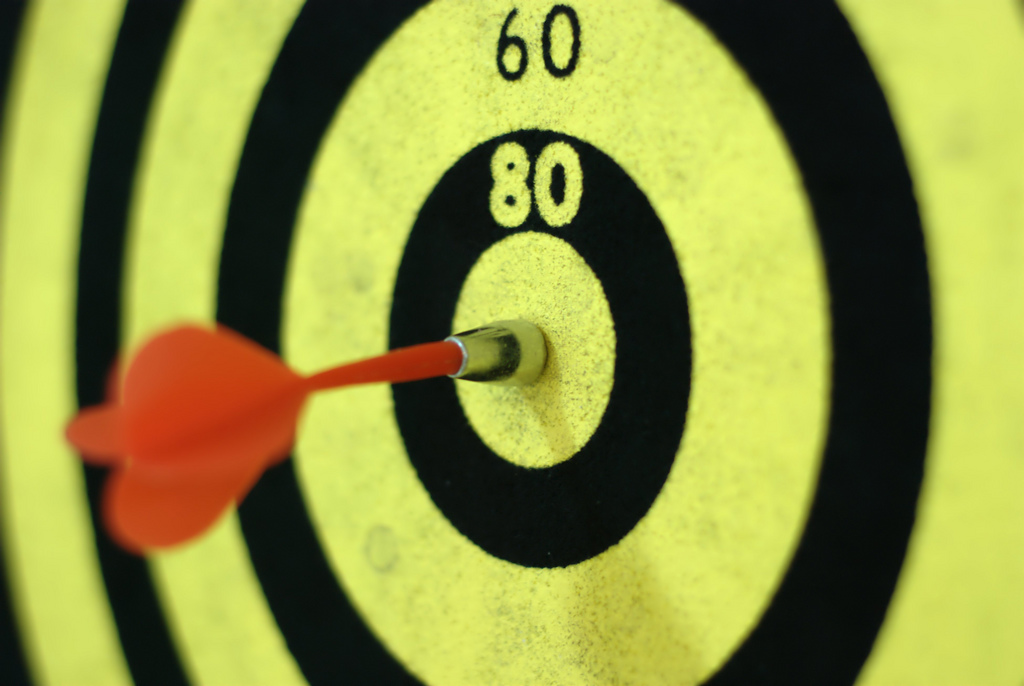
\includegraphics[height=\paperheight]{images/flickr_ogimogi_2223450729.jpg}}
\setbeamertemplate{footline}{\raisebox{2mm}[2mm][2mm]{\Tiny{https://www.flickr.com/photos/ogimogi/2223450729}{
      https://www.flickr.com/photos/ogimogi/2223450729}
    - CC-BY \href{https://www.flickr.com/photos/ogimogi}{Eran Sandler}}}
\begin{frame}
  \frametitle{}
  \begin{block}{}
    \begin{center}
      Our aims / wishes
    \end{center}
  \end{block}
\end{frame}

\begin{frame}
  \frametitle{}
  \begin{block}{}
    \begin{center}
      Raise the awareness for the\\relevance of research software.
    \end{center}
  \end{block}
\end{frame}

\begin{frame}
  \frametitle{}
  \begin{block}{}
    \begin{center}
      Include standards for research software into the common Good
      Scientific Practice recommendations.
    \end{center}
  \end{block}
\end{frame}

\begin{frame}
  \frametitle{}
  \begin{block}{}
    \begin{center}
      Introduce standards and mechanisms for quality control of
      research software.
    \end{center}
  \end{block}
\end{frame}

\begin{frame}
  \frametitle{}
  \begin{block}{}
    \begin{center}
      Create institutional platforms to publish and\\archive software/source
      code/workflows.
    \end{center}
  \end{block}
\end{frame}

\begin{frame}
  \frametitle{}
  \begin{block}{}
    \begin{center}
      Enable citation of such items.
    \end{center}
  \end{block}
\end{frame}

\begin{frame}
  \frametitle{}
  \begin{block}{}
    \begin{center}
      Make these citations part of the scientific reputation system.
    \end{center}
  \end{block}
\end{frame}

\begin{frame}
  \frametitle{}
  \begin{block}{}
    \begin{center}
      Foster the education of computational skills inside of the
      scientific community.
    \end{center}
  \end{block}
\end{frame}

\begin{frame}
  \frametitle{}
  \begin{block}{}
    \begin{center}
      Develop new carreer paths like\\ Research Software Engineers,
      Software Librarians, Data Scientists.
    \end{center}
  \end{block}
\end{frame}

\begin{frame}
  \frametitle{}
  \begin{block}{}
    \begin{center}
      Raise awareness about and teach legal aspects (i.e. licensing) of
      software.\\\
      \pause
      \\Make open source the default.
    \end{center}
  \end{block}
\end{frame}

\begin{frame}
  \frametitle{}
  \begin{block}{}
    \begin{center}
       Facilitate the transition from single-purpose solutions to
       application to services.
    \end{center}
  \end{block}
\end{frame}

\begin{frame}
  \frametitle{}
  \begin{block}{}
    \begin{center}
      Provide long-term funding to enable sustainable software
      development.
    \end{center}
  \end{block}
\end{frame}

\setbeamertemplate{background}{
  
\includegraphics[width=\paperwidth,trim=0 0 0 220,clip]{images/flickr_konrad_foerstner_4168966589.jpg}}
\setbeamertemplate{footline}{}
\begin{frame}
  \frametitle{}
  \begin{block}{}
    \begin{center}
      A lot to do and a lot of open questions.
    \end{center}
  \end{block}
\end{frame}

\setbeamertemplate{background}{
  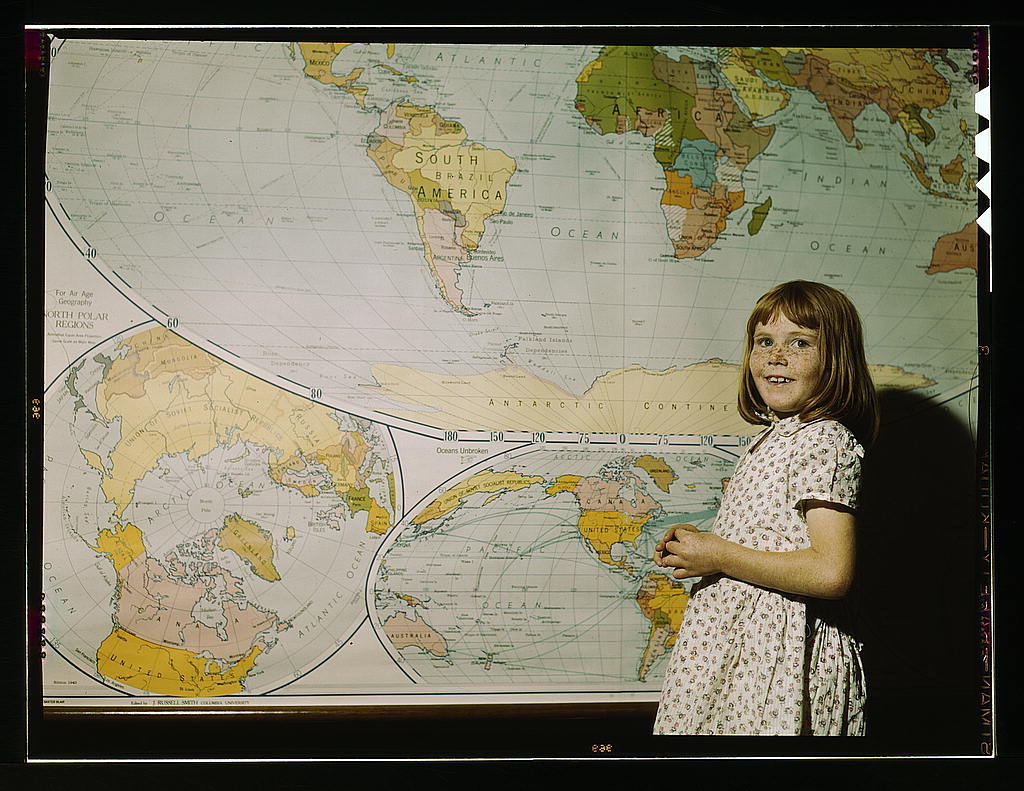
\includegraphics[height=\paperheight,trim=2 4 2 2,clip]{images/rural_school.jpg}}
\setbeamertemplate{footline}{\raisebox{2mm}[2mm][2mm]{
    \Tiny \href{http://www.everystockphoto.com/photo.php?imageId=2380666}{
      http://www.everystockphoto.com/photo.php?imageId=2380666} --
    The Library of Congress,  PD}}
\begin{frame}
  \frametitle{}
  \begin{block}{}
    \begin{center}
      We represent the German \\scientific community / research organisation.\\
      \ \\
      \pause
      Ideally all these issues are adressed on an international level.
    \end{center}
  \end{block}
\end{frame}

\setbeamertemplate{background}{
  \includegraphics[width=\paperwidth,trim=1 1 1 1,clip]{images/1024px-Pierre_Pénicaud_-_Plaque_with_Acrobats_-_Walters_44189.jpg}}
\setbeamertemplate{footline}{\raisebox{2mm}[2mm][2mm]{
   \Tiny \href{https://commons.wikimedia.org/wiki/File:Pierre_P\%C3\%A9nicaud_-_Plaque_with_Acrobats_-_Walters_44189.jpg}{https://commons.wikimedia.org/wiki/File:Pierre\_P\%C3\%A9nicaud\_-\_Plaque\_with\_Acrobats\_-\_Walters\_44189.jpg} PD}}
\begin{frame}
  \frametitle{}
  \begin{block}{}
    \begin{center}
      Let's do this together!
    \end{center}
  \end{block}
\end{frame}

\setbeamertemplate{background}{
  
\includegraphics[height=\paperheight]{images/flickr_nateone_3768979925.jpg}}
\setbeamertemplate{footline}{\raisebox{2mm}[2mm][2mm]{
    \Tiny {\url{http://www.flickr.com/photos/nateone/3768979925/} 
      -- CC-BY by flick user \href{http://www.flickr.com/photos/nateone/}{nateone}}}}
\begin{frame}
  \frametitle{}
  \begin{block}{}
    \begin{center}
      \includegraphics[height=2cm]{images/logo_allianz.png}\\
      \vspace{1.5cm}      
      \textbf{\href{http://www.allianzinitiative.de/}{www.allianzinitiative.de}}\\
      \vspace{1.5cm}
      \href{http://twitter.com/konradfoerstner}{@konradfoerstner}
      \end{center}    
  \end{block}
\end{frame}

\end{document}
